\subsection{Process 1: Public Transport Handler}
\label{subsec:process_1}
One integral functionality within our Networked Traffic Control System involves the seamless integration of public transport vehicles, such as buses and trams, with the capability to communicate effectively with the TCU. Specifically, a noteworthy feature of our system is the ability of public transport vehicles to initiate communication with the TCU, thereby requesting an extension of the signal duration. This communication process is crucial for optimizing traffic flow. To elaborate on the mechanism, the public transport vehicle initiates the interaction by transmitting a signal to the TCU, requesting for an extended signal time.The process works as follows:
\begin{itemize}
\item In the initial phase, the TCU undergoes a verification process to determine if it has received any input from a public transport vehicle. In the absence of any input, the TCU diligently continues to monitor for incoming signals.
\item Upon receiving an input, the TCU conducts a further assessment to verify if the vehicle input received from the ROW corresponds to the signal associated with the requested ROW extension. This stringent matching process ensures that the request aligns precisely with the anticipated response. In instances where a match is not successfully established, the current request is promptly discarded, and the TCU resumes its vigilance for new inputs.
\item In the event of a successful match, the TCU proceeds to evaluate the possibility of extending the signal time. If the conditions allow for an extension, the TCU seamlessly executes the signal time extension. Conversely, if an extension is not permissible based on the existing criteria, the current request is promptly discarded, and the TCU resumes its continuous monitoring for any subsequent input.
\end{itemize}
\begin{figure}
\centering
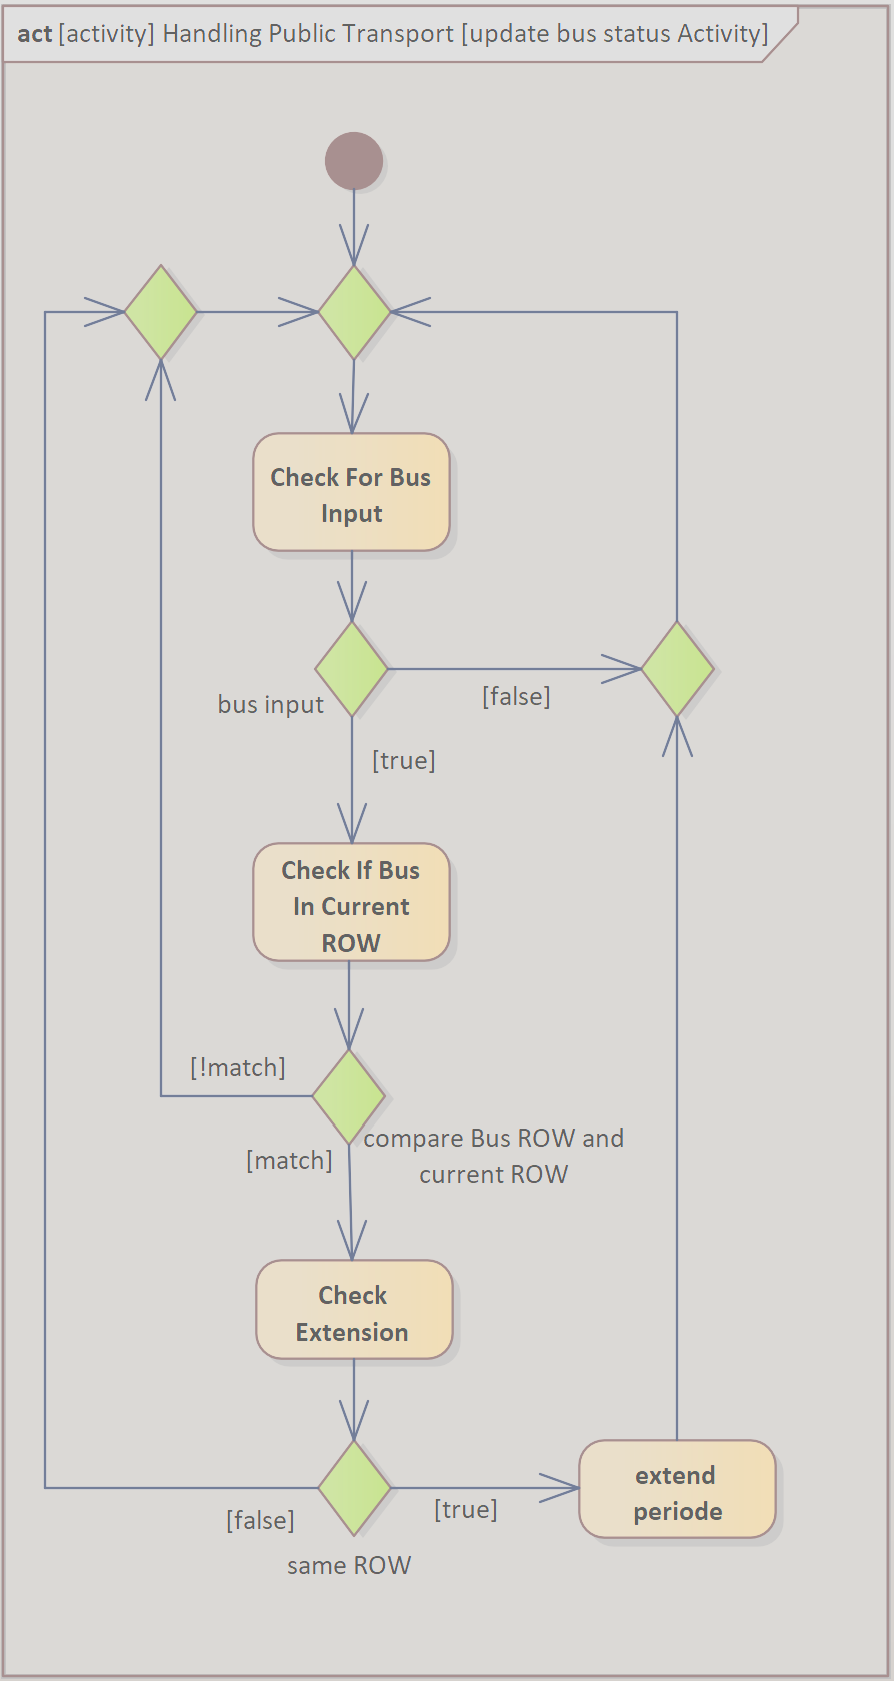
\includegraphics[width=0.5\linewidth]{images/process_1_activity.png}
\caption{Public Transport Integration (Bus) Activity}
\label{fig:bus_listener}
\end{figure}
The interaction between the public transport vehicle and TCU encompasses the dynamic adjustment of the idle scheduling within the traffic system as shown in Figure 8. Initiated by the Bus Listener, the process unfolds as follows: upon receiving input, the Bus Listener transmits a signal request to the TCU. Subsequently, the TCU engages in processing this signal request, evaluating the decision to be made.In instances where a signal extension is requested and deemed appropriate, the TCU issues a message instructing the adjustment of the signal schedulers behavior. This adjustment is based on the specified signal extension time. 
\begin{figure}
\centering
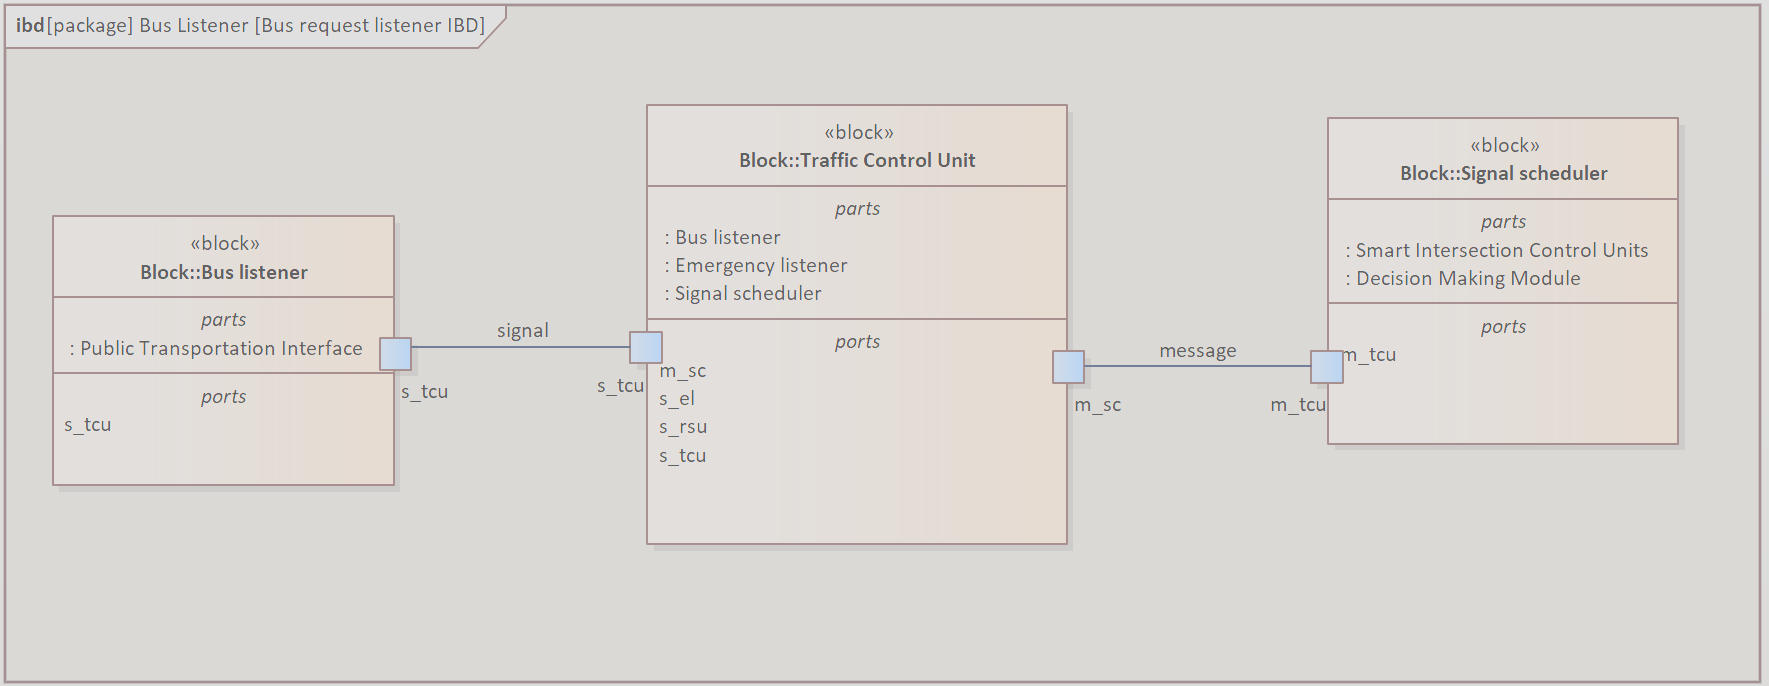
\includegraphics[width=1\linewidth]{images/bus_listener_ibd.png}
\label{fig:bus_listeneribd}
\caption{Interaction between Bus Listener and Signal Scheduler through TCU}
\end{figure}